\documentclass[titlepage,a4paper,11pt]{article}
\usepackage[pdfborder={0 0 0}]{hyperref}
\usepackage{fontspec}
\usepackage[hmargin=2.54cm,vmargin=1.91cm]{geometry}
\usepackage{parskip}
\usepackage{wrapfig}
% TableMagic+shading
\usepackage{multirow}
\usepackage[english]{babel}
\usepackage{longtable}
\usepackage{float}
\usepackage{graphicx}
\usepackage[table]{xcolor}
\definecolor{tableShade}{HTML}{F1F5FA}

\def \project {Defense of the Guardian Gnome}
\def \objective {guardian gnome}

\setromanfont{Century Gothic}

\date{\today}

\begin{document}
\title{Artitectural Description Document\\
 		TDT4240 - XNA Game Project}

\author{Dag Øyvind Tornes\\
 		Sibte-Haider Syed\\ 
		Robin Kåveland Hansen\\}
\maketitle

\pagestyle{empty}
\tableofcontents
\clearpage
\pagestyle{plain}
\pagenumbering{arabic}

\section{Introduction}
This document describes the requirements that have been developed for \project,
a game developed for the XNA platform. It describes the functional requirements
and thus a high-level overview of how the game should play. There are also some
scenarios for content development that describe the quality requirements imposed
on the system. Chapter \ref{concepts} describes the concept behind the game on
a high level, as well as some discussion around some game design choices that
have been made at this time or will have to be made in the future. Chapter
\ref{funcreq} lays down the functional requirements that were decided on.
Chapter \ref{qualreq} deals with the quality requirements in detail, as well as
some scenarios that might be relevant for \project. Chapter \ref{constraints}
describes in some detail the constraints that were imposed on the game by either
the developers, or the technology used.


\section{Architectural Drivers}
We have identified the following drivers as most important to our project:
\begin{itemize}
	\item Due to the time constraint on this project we wish to create an 	
	architecture which is as modifiable as possible, to allow quick iterations
	in development.
	\item A game of this nature needs to be balanced in such a way to keep it
	hard enough for seasoned players, and accessible to newcomers.  Thus we 
	wish to keep the architecture data-driven in all areas, allowing us to
	change constants and tweak difficulty quickly.
\end{itemize}

\section{Stakeholders and Concerns}
\subsection{Developers}
Members:  Dag Øyvind Tornes, Sibte-Haider Syed, Robin Kåveland Hansen

Concerns: The developers primary concern is to create a game which is 
enjoyable, while still satisfying the course requirements, and receiving a
good grade.  Also, we would like to not work ourselves to death.

\subsection{Evaluators}
Members:  The ATAM team and teaching staff.

Concerns: The evaluators will be concerned with a cleanly designed and well
documented architecture, as this is their primary view of the game.  They will
probably also want to see an implementation in sync with the documentation.

\subsection{The players}
Members:  The development team, and other parties looking for a lot of fun.

Concerns:  The players will want a game which is easy to learn, and fun to
play.  

\section{Selection of Architectural Viewpoint}
\subsection{Logical View}

\begin{table}[H]
	\resizebox{\textwidth}{!}{
	\rowcolors{0}{white}{tableShade}
	\begin{tabular}{p{5cm} | p{12cm}}
    	\hline
		\textbf{Objective}		&	Describes the functionality of the system with a modeling language \\															
		\textbf{Notation}		& 	Implied by the chosen modeling language \\ 
		\textbf{Stakeholder}	& 	Testers, evaluators and developers	\\
		\textbf{Selection}		& 	Class diagrams \\
		\hline
    \end{tabular}
	\label{tab:log_view}}
\end{table}

\subsection{Process View}

\begin{table}[H]
	\resizebox{\textwidth}{!}{
	\rowcolors{0}{white}{tableShade}
	\begin{tabular}{p{5cm} | p{12cm}}
    	\hline
		\textbf{Objective}		&	Describes non-functional requirements constraining performance, 
									concurrency, integrity and availability. \\															
		\textbf{Notation}		& 	State, Activity and sequence diagrams \\ 
		\textbf{Stakeholder}	& 	Evaluators and developers	\\
		\textbf{Selection}		& 	Sequence diagrams \\
		\hline
    \end{tabular}
	\label{tab:process_view}}
\end{table}

\subsection{Development View}

\begin{table}[H]
	\resizebox{\textwidth}{!}{
	\rowcolors{0}{white}{tableShade}
	\begin{tabular}{p{5cm} | p{12cm}}
    	\hline
		\textbf{Objective}		&	Describes the system by modules and subsystem diagrams, 
									showing the ‘export’ and ‘import’ relationships. \\															
		\textbf{Notation}		& 	Booch \\ 
		\textbf{Stakeholder}	& 	Evaluators and developers	\\
		\textbf{Selection}		& 	None at this iteration \\
		\hline
    \end{tabular}
	\label{tab:dev_view}}
\end{table}

\subsection{Physical View}

\begin{table}[H]
	\resizebox{\textwidth}{!}{
	\rowcolors{0}{white}{tableShade}
	\begin{tabular}{p{5cm} | p{12cm}}
    	\hline
		\textbf{Objective}		&	Describes the the non-functional requirements of 
									the system such as availability, reliability 
									(fault-tolerance), performance (throughput), and 
									scalability.  \\															
		\textbf{Notation}		& 	Physical blueprints \\ 
		\textbf{Stakeholder}	& 	Not relevant, available if needed\\
		\textbf{Selection}		& 	None, not relevant \\
		\hline
    \end{tabular}
	\label{tab:Physical view}}
\end{table}

\subsection{Scenarios}

\begin{table}[H]
	\resizebox{\textwidth}{!}{
	\rowcolors{0}{white}{tableShade}
	\begin{tabular}{p{5cm} | p{12cm}}
    	\hline
		\textbf{Objective}		&	To use the other views and create scenarios which 
									works towards validating the architectural choices	\\															
		\textbf{Notation}		& 	Scenarios, Scenario diagrams \\ 
		\textbf{Stakeholder}	& 	All\\
		\textbf{Selection}		& 	Scenarios \\
		\hline
    \end{tabular}
	\label{tab:scenario_view}}
\end{table}

\section{Architectural Tactics}
\subsection{Availability Tactics}
\begin{itemize}
	\item Handle battery failure of Xbox-controller by pausing game and
	allowing resuming later.
\end{itemize}

\subsection{Modifiability Tactics}
\begin{itemize}
	\item The architecture should be as modular as possible, with 	
	the responsibilities of each module clearly delineated.  This should
	localize changes to the system to the greatest possible degree.
	\item By using a data-driven approach, the architecture should be well
	suited for fast changes.
	\item Component-based game logic.  Each entity in the game, be it the
	player or a puff of smoke, should be made up from small components with
	clear responsibilities.  This should allow quick changes to gameplay at
	a late date, and allow us to add new functionality without affecting
	existing code.
\end{itemize}

\subsection{Usability Tactics}
\begin{itemize}
	\item The game should have a clean and simple graphical style, and should
	not confuse the player with needless complexity.
	\item The interface should follow Microsofts UI-guidelines as much as 
	possible.
	\item By using the Model-View-Controller pattern we hope to achieve a 
	simple architecture to drive the application.
\end{itemize}

\subsection{Performance Tactics}
\begin{itemize}
	\item Profile then optimize.
	\item Decouple rendering and game logic.
\end{itemize}

\subsection{Security Tactics}
\begin{itemize}
	\item Not relevant to this project
	\item Non-networked games can be considered \quote{trusted}
\end{itemize}

\subsection{Testability tactics}
\begin{itemize}
	\item The game should monitor internal state, and allow reporting this
	in a debug-mode for developers.
	\item Unit-tests should be employed as extensively as possible
\end{itemize}

\section{Architectural Patterns}
\subsection{Model View Controller}
The Model View Controller pattern (MVC) is a way of dividing an application
into clear and separated responsibilities. MVC is not perfectly suited to 
games, but we will be using some of the ideas behind it to achieve modularity.

The problem with using MVC in a game is that views, i.e. a camera, are closely
related to the game itself, which represents the model.  Controller is also 
not easily fitted in this particular game, due to the way XNA handles IO.

Our solution is to separate out as much of the view as possible in a separate
renderer module.  This will need some knowledge of the game, but we hope to 
minimize this by creating general methods which may be applied in several 
contexts.

\subsection{Event-driven programming}
While event-driven programming is not strictly a pattern, it is such a big 
part of our architecture we feel it should be mentioned here.

The thinking behind our version of this is to split functionality in the game
into small components which know how to handle a small set of events, and 
achieving more complex features through interaction between these components.

\subsection{Component-based entities}
Entities are anything and everything which appears in-game.  This includes the
player, creeps and the level.  We hope to make these parts as interchangeable 
as possible by using a component-based system for entities.  The idea is that
functionality can be composed of small reusable components which can interact.
This is the approach taken in Unity, one of the most popular game-engines for 
the Windows and Mac platforms.

\section{Views}
\subsection{Logical View}

\begin{figure}[H]
	\begin{center}
		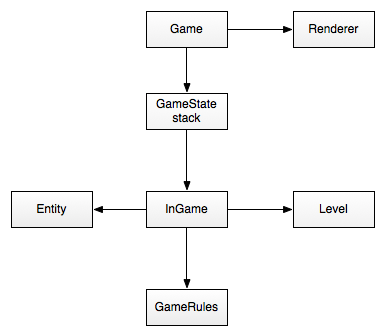
\includegraphics[scale=0.75]{graphics/DataManagementView}
	\end{center}
        \caption{Box and arrow diagram of game classes}
\end{figure}

The box and arrow diagram shows which modules and components that will be
used to implement the design. XNA assumes a Game class as the entry point of
the application, so this will be where everything starts. Aside from that,
we clearly need a DataManager to facilitate a data-driven application. The
idea here is that the DataManager will be able to import all kinds of data that
may be required by other components of the game, such as sprites, hero statistics,
levels and so on. It should also be able to store and retrieve a highscore list.

The GameState stack is how the game keeps track of what it should be doing right
now. For example, assuming the player pushes Start to pause the game, what should
happen is that a Paused state is pushed onto the stack, and then popped whenever
the player is done pausing. This is where menus and the like are handled.

We have decided that a Renderer is desirable, so that we can switch around on how
the graphics are handled at a later date. To facilitate this, we implement a
uniform interface for how an object can get itself rendered to the screen, and
an instance of a Renderer of some sort is passed down the call-chain down to the
entities that wish themselves to be rendered. In other words, this enables us to
not have to define how objects are Rendered in the objects themselves, and should
enable us to easily change graphical styles and the likes late in the development
cycle.

Ingame is the class that handles everything game-mechanical, directly or
indirectly. This is where the game-loop takes place. It has access to an Event
system, currently envisioned to incorporate an EventQueue class, and an Event
class. Ingame objects are allowed to push Events onto the EventQueue. Using
Events allows us to skip defining trigger methods of various kinds on all the
objects in the game, and makes the game semi-scriptable, enabling us to quickly
add different kinds of behaviour for creeps, projectiles and everything else.
Instead of having triggers then, the various objects have EventHandlers, if
they are so inclined.

Movable, collidable objects are Entities. Heros and creeps are subclasses
of this class, as is Particle, which has a slightly different behaviour.
\subsection{Process View}

\begin{figure}[H]
	\begin{center}
		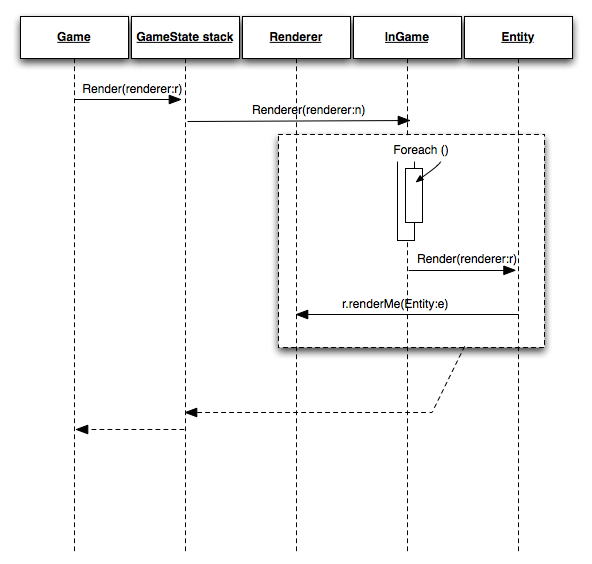
\includegraphics[scale=0.75]{graphics/GameRendersToScreen}
	\end{center}
        \caption{Game renders to screen}
\end{figure}

We have chosen to include 3 sequence diagrams that show the interactions between
components in some illustrative situations here. The first one shows how Rendering
of ingame objects takes place. The Game wants to render to screen, and so it
tells the GameState stack, and passes along a Renderer which it can use for this
purpose. The Game class does not need to be aware of which state the Game is in
to do this. The GameState stack knows that it is currently in a game, and so
it delegates this task to the Ingame class. This class iterates over all its
renderable objects, and tells them to render with the Renderer that was passed
down the call-chain. These then give the Renderer information about where they
are, and the Renderer does the rest.

\begin{figure}[H]
	\begin{center}
		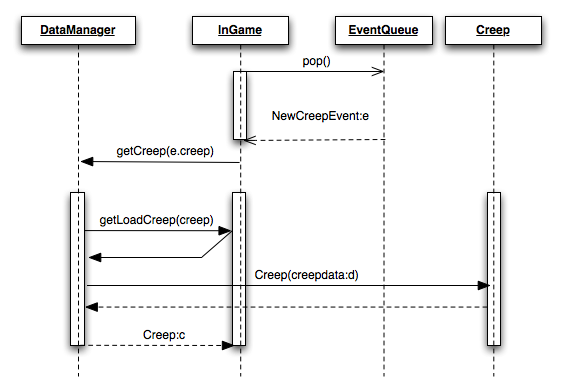
\includegraphics[scale=0.75]{graphics/GameSpawnsCreep}
	\end{center}
        \caption{Game spawns creep}
\end{figure}

The second one shows how creeps are spawned. At some point, a SpawnCreep event
was added to the EventQueue (Probably by the Level), and this event should now
be triggered as discovered by the EventQueue. Ingame polls the EventQueue,
and gets this event in return. It asks the DataManager for information about this
creep, and the DataManager discovers that it hasn't loaded this creep type yet, so
it has to fetch the data from the storage system. Once this is done, it
creates an instance of the creep type and sends it back to Ingame.

\subsection{Player Shoots}
\begin{figure}[H]
	\begin{center}
		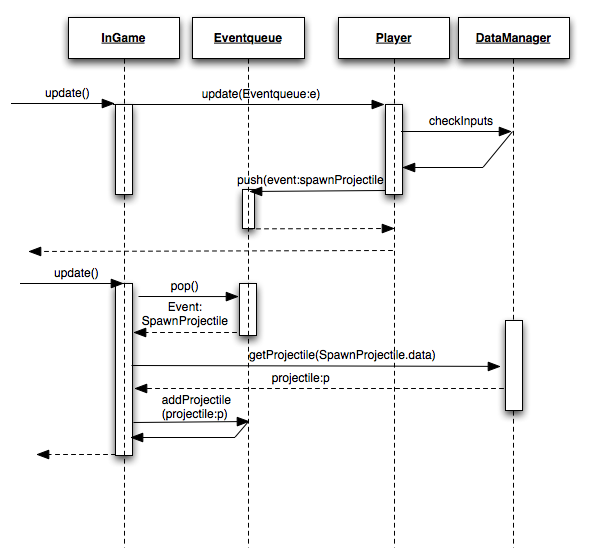
\includegraphics[scale=0.75]{graphics/PlayerShoots}
	\end{center}
        \caption{Player shoots}
\end{figure}

The third one details what happens when a player shoots. The essential of the
situation is that a player checks its input, and finds the shoot button to be
pressed. This causes it to create a PlayerShootsEvent, which is pushed to the
EventQueue. Next iteration of the game update loop causes this event to be
popped and processes, spawning a Projectile in the end. When this projectile
collides with something, it can create a CollisionEvent causing the game
to update health and draw a nice explosion or something similar.

\subsection{Scenarios}

\begin{figure}[H]
	\begin{center}
		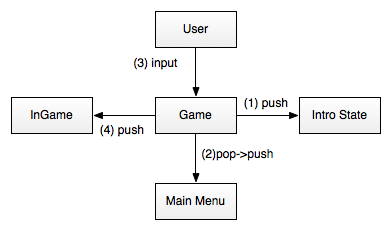
\includegraphics[scale=0.75]{graphics/scenario_1_StartingGame}
	\end{center}
        \caption{Game is started}
\end{figure}

Scenario 1 details which components that interact when a game is started. Scenario
2 details what takes place once a player dies, and achieves a new highscore.

\begin{figure}[H]
	\begin{center}
		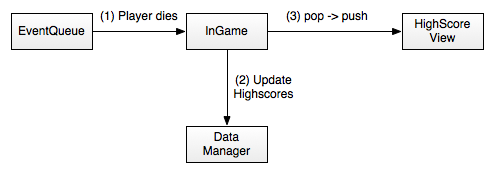
\includegraphics[scale=0.75]{graphics/scenario_2_PlayerDiesHighScore}
	\end{center}
        \caption{Player dies, and achieves a highscore}
\end{figure}


\section{Consistency Among Views}

\section{Architectural Rationale}

%\section{Issues}

\section{References}

\end{document}
